\section{XSnare Design} \label{xsnare_design}

 \begin{figure}[h]
	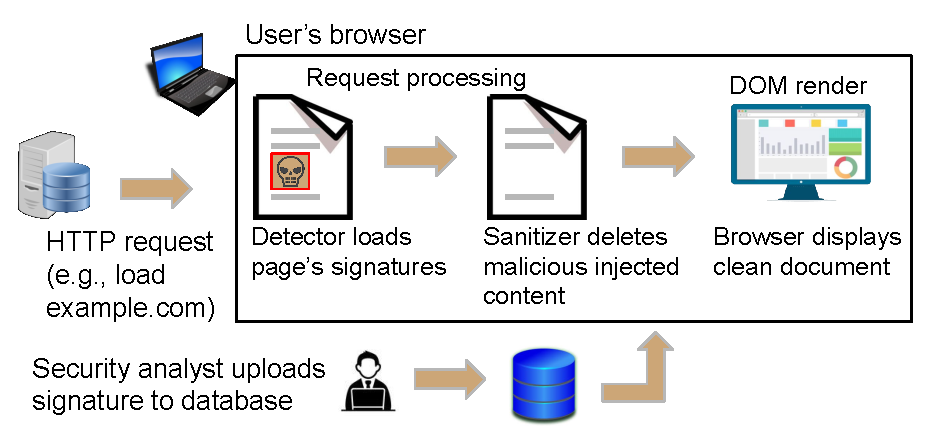
\includegraphics[scale=0.55]{img/xsnare.pdf}
	\caption{\sys's approach to protect against XSS.}
	\label{fig:xsnare}
\end{figure}

We now introduce \sys and its components. % and how they interact with each other.
%
% \subsection{Operation, at a glance} \label{operation}
%
Figure~\ref{fig:xsnare} illustrates how the firewall can be used to
guarantee full client-side XSS protection: A user loads a request,
such as \url{www.example.com}, this request might come back with
malicious code in the form of an XSS attack. Before rendering the
webpage in the browser, an extension can analyze the potentially
malicious document. First, it loads signatures which a security
analyst
%% (a bug bounty hunter, for example)
has uploaded to a database. The extension's detector analyzes the
given HTML string and identifies the signatures which apply to this
document. The signatures specify the injection spots in the document,
and the extension's sanitizer gets rid of any malicious
content. Finally, the extension passes a clean HTML document to the
browser for rendering. Algorithm \ref{filter_algorithm} describes the
network filtering process. Section \ref{implementation} explains this
algorithm in more detail.
 
\subsection{An example application of \sys} \label{motivating_example}

To further explain our approach, we present a small example of how
DOM context can be used to defend against XSS, taken from CVE
2018-10309~\cite{examplecve}. This is reproducible in an off-the-shelf
WordPress installation running the Responsive Cookie Consent plugin,
v1.7. This is also an example exploit which Chrome's XSS auditor does
not protect against. Consider a website running PHP on the backend
that takes user input and stores it to later display it to another
user; in this case, the \textbf{input} element's value.

The PHP code defines the static HTML template (in black), as well as the dynamic input (in red):

\begin{lstlisting}
<input id="rcc_settings[border-size]" 
name="rcc-settings[border-size]" 
type="text" value=<@\textcolor{red}{"<?php rcc\_value('border-size'); ?>"}@>/>
<label class="description"
for="rcc_settings[border-size]">
\end{lstlisting}
Under normal circumstances, the \textbf{input} might have a value of "0":
\begin{lstlisting}
<input id="rcc_settings[border-size]" 
 name="rcc-settings[border-size]" 
 type="text" value=<@\textcolor{red}{"0"}@>>
<label class="description"
 for="rcc_settings[border-size]">
\end{lstlisting}
However, the php code is vulnerable to an injection attack, e.g.:
\begin{lstlisting}
border-size = ""><script>alert('XSS')</script>
\end{lstlisting}
The browser will render the following, executing the injected script:
\begin{lstlisting}
<input id="rcc_settings[border-size]" 
name="rcc-settings[border-size]" 
type="text" value=<@\textcolor{red}{""><script>alert('XSS')</script>}@>
<label class="description"
for="rcc_settings[border-size]">
\end{lstlisting}

Note that this HTML is well-formed, so it is hard to detect that a malicious injection has occurred without knowing the application developer's intention. However, assuming an analyst has knowledge of how the full HTML should render without any injections, they can single out the point of injection, by separating the dynamic content from the server-side template, and get rid of the malicious script entirely. In the example, the injected script can be easily distinguished from the rest of the HTML template due to their identifiable attributes. By searching for this specific \textbf{input} element from the top of the document, and this \textbf{label} element from the bottom, we can effectively ensnare injection points in the HTML. 

This mechanism is partly inspired by work from Nadji et al.~\cite{Nadji:2009}. Their client and server-side hybrid approach for XSS defence, uses server-specified policies enforced on the client side. Unlike other prior work, they do not rely on developers to identify untrusted sources, and tag elements server-side, such that the client has a clear distinction of untrusted code, which can be filtered accordingly. We remove the server-side component by tagging client-side.

When sanitizing the injection points, we would ideally apply functions that are equivalent to the server-side patch, but the application developer's intention might not always be clear. We analysed the code in the example, and we noted that while the developer claimed the bug was fixed in version 1.8 of this plugin, this was not the case: the developer fixed other similar vulnerabilities but did not handle this specific parameter. However, we can infer the application's intended behaviour from the other patches~\cite{rccpatch}. In particular, the developer applied a built-in WordPress function \code{sanitize\_text\_field}, which sanitizes the parameters by checking for common invalid characters like invalid UTF-8. The task of determining the intended behaviour falls upon a security analyst, who will act as the signature developer for a given exploit.  

In the following sections we give a detailed description of each component of our system, the challenges that arise when trying to defend against XSS client-side, and the tools provided by the browser to facilitate our methods. 

\subsection{\sys Signatures} \label{signatures}
The signatures are at the core of XSnare. They must be precise enough for our system to get rid of the intended injection, without removing elements of the website crucial to the user experience. Since we are only relying on DOM knowledge, these signatures must be related to HTML features, for example, specifying elements and attributes that are unique to where the exploit might occur. 

The basis for our signatures relies on two observations: first, \textbf{an injection must have a start point and end point}, that is, an element can only be injected between a specific HTML node and its immediate sibling in the DOM tree; second, in a well-formed DOM, \textbf{the dynamic content will not be able to rearrange its location in the document without JavaScript execution} (e.g., removing and adding elements), allowing us to isolate it from the template code. Thus, our basic approach at signature definition is to specify an injection's start and its end, and any sanitization to be done between these two endpoints. Typically, one page will have several dynamic content injection points. We discuss the difficulties that arise when this occurs and the techniques we used to deal with these in later sections.

We believe CVEs to be an ideal source for signatures. Since previous client-side work does not focus on application-specific protection, these tools often use less accurate heuristics to detecting exploits. Furthermore, once new vulnerabilities are found, these systems often lack the maintainability obtained by leveraging active CVE development. 

%Our system assumes signatures are written by a third-party: 
Bug bounty hunters and penetration testers will commonly identify issues in application code, inform developers and publish them for the benefit of the community in the form of CVES.

We require an extra step in the workflow, which is to audit CVEs and convert them into corresponding signatures. Security enthusiasts and web developers would have the competency to fulfil this role and propose new signatures (i.e. they have working knowledge of the page's HTML ). We imagine that an organisation would vet these proposals and gather them into an audited database, akin to how antivirus or antispam software is managed.

%Thus, the signature database is maintained by a trusted entity which audits CVEs, and a malicious analyst cannot take advantage of this model to harm the user's browsers through signatures. An analyst can write a signature in our language given their knowledge of the exploit, as they will often know both the source and the way it manifests in the HTML, as well as the fix.
 
 \subsection{Firewall Signature Language} \label{signature_language}
 Our signature language needs to be such that it has enough power of expression for the signature writer to be precise, both for determining the correct web application and to identify the affected areas in the HTML. For injection point isolation, a language based on regular expressions (regex language) suffices to express precise sections of the HTML. The following is the signature that defends against the motivating example of Section 2.2:
\begin{lstlisting}[breaklines=true,caption={An \sys signature},label={lst:xsnare_signature}]
url: 'wp-admin/options-general.php?page=rcc-settings',
software: 'WordPress',
softwareDetails: 'responsive-cookie-consent',
version: '1.5',
type: 'string',
typeDet: 'single',
sanitizer: 'regex',
config: '/^[0-9](\.[0-9]+)?$/',
endPoints: 
['<input id="rcc_settings[border-size]" name="rcc_settings[border-size]" type="text"
  value="',
'<label class="description" 
for="rcc_settings[border-size]">']
\end{lstlisting}

A description of the development process for this signature is given in Section \ref{case_study}. In summary, a signature will have the necessary information to determine whether a loaded page has a vulnerability, and the HTML identifiers to properly eliminate malicious content.
  
Once the page's identifying information and the dynamic content is established by an analyst, they can configure their signatures with a function chosen from a pre-defined static set of sanitization functions. These functions inoculate potentially malicious injections based on the DOM context surrounding the injection. The goal of signatures is to provide such sanitization, while maintaining the core web page user experience. To this end, default injection point sanitization is done with DOMPurify's  ~\cite{10.1007/978-3-319-66399-9_7} default configuration~\footnote{This library is described by its creators as a "DOM-only, super-fast, uber-tolerant XSS sanitizer for HTML, MathML and SVG". The Mozilla community cites it as an useful tool for "safely inserting external content into a page"~\cite{safecontent}}. However, there are cases where page functionality is lost due to a generic sanitization approach. Thus, a different sanitization method can sometimes be more desirable.
  
An alternative to providing static functions would have been to allow signatures to
specify arbitrary code for the sanitization routines. While this would
provide more accurate sanitization, we have decided to
impose a declarative spec for security reasons and because we believe
a declarative spec is sufficiently expressive.

%% \begin{enumerate} 
%% 	\item Security Concerns: We assume signatures come from a trusted source. However, partly due to the way they are currently stored, it is possible for an attacker to add malicious signatures. In general, this would only harming the web site user experience by removing safe content. The ability to run arbitrary code would lead a serious security flaw, as it would execute in a high-privilege environment.
%% 	\item Case Coverage: While our provided methods might be limited in some scenarios, we have applied them in our studied CVEs with positive results, and are confident they can cover most use cases.
%% 	\item Adoption: A declarative language will help signature developers expedite the process of writing signatures, as they will find that our provided methods will most often suffice.
%% \end{enumerate}
 
 \subsection{Firefox Extension} \label{firefox_extension}
 Our system's main component is a browser extension which rewrites potentially infected HTML into a clean document. We believe an extension to be ideal for our purposes due to the context available to it. Previous client-side work has focused on browser modifications and higher-level tools. These tools do not have the context required for the application-specific behaviour we seek. The extension detects exploits in the HTML by using signature definitions and maintains a local database of signatures that is periodically updated from the main server. The extension translates signature definitions into patches that rewrite incoming HTML on a per-URL basis, according to the top-down, bottom-up scan described in \autoref{motivating_example}. 

The patch applied by the extension needs to take place in the raw HTML string: even before any code runs, parsing the HTML into a DOM tree might cause elements to be re-arranged into an unexpected order, making our extension sanitize the wrong spot. 
Consider the following example, where an element inside a <tr> tag is rearranged after parsing the string:

\begin{lstlisting}
<table class="wp-list-table">
  <thead>
     <tr>
	     <th></th>
	     <@\textcolor{red}{<img src="1" onerror="alert(1)">}@>
	     <th>
   	     <form method="GET" action="">
...
\end{lstlisting}

In this HTML, the signature developer might identify the exploit as occurring inside the given table. However, if we wait until the string has been parsed into a DOM tree to sanitize, the elements are rearranged due to <tr> not allowing an <img> as its child:

\begin{lstlisting}
<@\textcolor{red}{<img src="1" onerror="alert(1)">}@>
<table class="wp-list-table">
   <thead>
   <tr>
	   <th></th>
	   <th>
       <form method="GET" action="">
...
\end{lstlisting}

Note that the injected <img> tag is now outside of the table, simply by virtue of the DOM parsing. Now, the extension will search past the injection, as it occurs before the table element, creating a false negative (FN). Similarly, elements rearranged inside an injection point can create false positives. This example would generate a class of circumvention techniques for our detector, so we can't wait until the website has been rendered to analyse the response, and therefore, our detector acts as an in-browser network filter. This guarantees that a knowledgeable attacker can not take advantage of this behaviour.

\subsection{Handling multiple injections in one page} \label{multiple_injections}
In Listing \ref{lst:xsnare_signature}, the endPoints were listed as two strings in the incoming network response. However, there are cases where arbitrarily many injection points can be generated by the application code, such as a for loop generating table rows. For these, it is hard to correctly isolate each endPoint pair, as an attacker could easily inject fake endPoints in between the original ones.

\begin{figure}[h]
	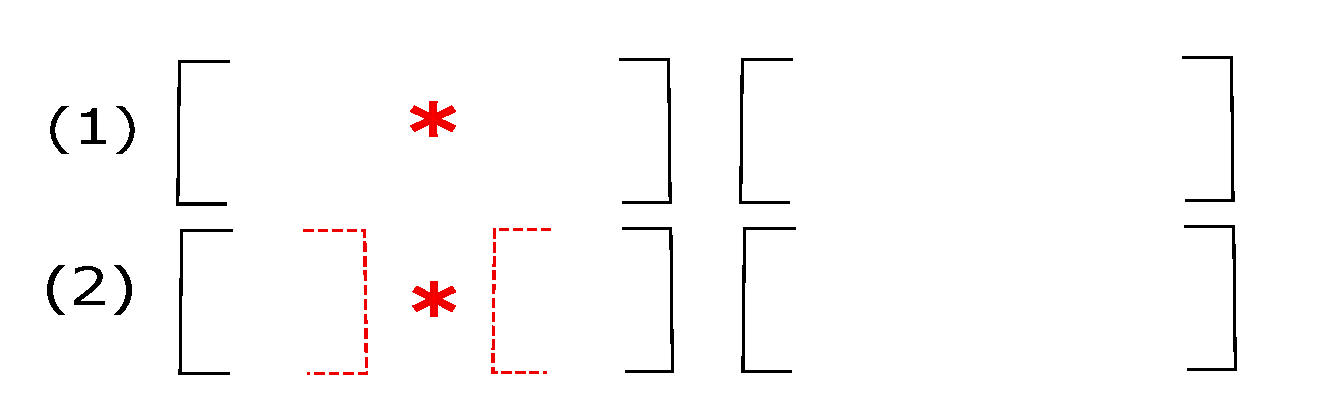
\includegraphics[scale=0.25]{img/attacker_injection_compound.pdf}
	\caption{Example attacker injection when multiple injection points exist in the page. a) a basic injection pattern. b) an attempt to fool the detector.}
	\label{fig:attacker_injection}
\end{figure}

In Figure~\ref{fig:attacker_injection}a, the brackets indicate a template. The content in between is an injection point (the star), where dynamic content is injected into the template. In the case of a vulnerability, the injected content can expand to any arbitrary string. The signature separates the injection from the rest by matching for the start and end points (the \code{endPoints}), represented by the brackets. This HTML originally has two pairs of \code{endPoint} patterns.

In Figure~\ref{fig:attacker_injection}b, the attacker knows these are being used as injection end points and decides to inject a fake ending point and a fake starting point (the dotted brackets), with some additional malicious content in between. If just looking for multiple pairs of end points, the detector cannot tell the difference between the solid and dotted patterns, and will not get rid of the content injected in the star. Therefore, we have to use the first starting point and the last ending point before a starting one (when searching from the bottom-up) and sanitize everything in between. This might get rid of a substantial amount of valid HTML, so we defer to the signature developer's judgement of what behaviour the detector should follow. We expand upon this further in \autoref{case_study}.


\begin{figure}[h]
	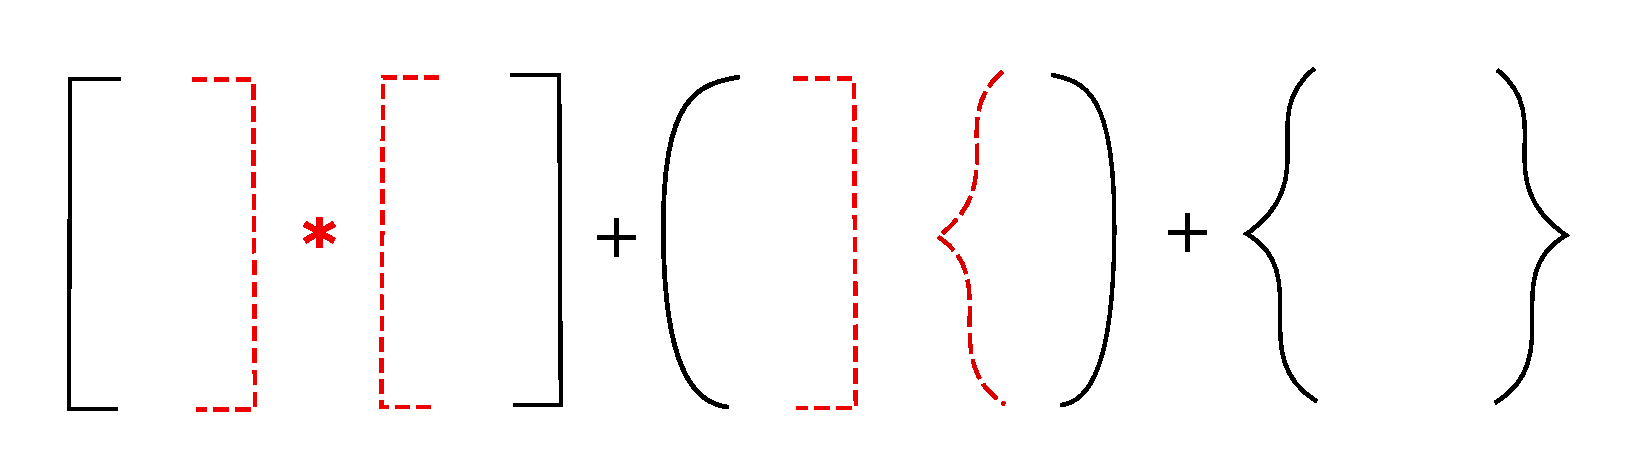
\includegraphics[scale=0.25]{img/attacker_injection_unique.pdf}
	\caption{Example attacker injection when multiple distinct injection points exist in the page.}
	\label{fig:attacker_injection_unique}
\end{figure}


Figure ~\ref{fig:attacker_injection_unique} illustrates a case when there are several injection points in one page, but each of them is distinct. Now, the filter is only looking for one pair of brackets, so the attacker can't fool the extension into leaving part of the injection unsanitized. However, they could, for example, inject an extra ending bracket after the opening parenthesis (or an extra starting brace). The extension will be tricked into sanitizing non-malicious content, the black pluses (+). This behaviour can be detected by noting that we know the order in which the \code{endPoints} should appear, and so if the filter sees a closing \code{endPoint} before the next expected starting \code{endPoint}, or similarly, a starting \code{endPoint} before the next expected closing \code{endPoint}, this attack can be identified. In the diagram, the order of the solid elements characterizes the possible malformations in the end points. As with the previous scenario, we have to sanitize the outermost end points, potentially deleting non-malicious content. The signature developer specifies the sanitization behaviour.

\subsection{Dynamic injections} \label{dynamic_injections}

The top-level documents of web pages fetch additional dynamic content
via \js{fetch} or AJAX APIs. Content fetched in
this way is also vulnerable to \xss, and must be filtered. An example
vulnerability is CVE-2018-7747 (Wordpress Caldera Forms, which allows malicious
content retrieved from the plugin's database to be injected in response to a click.

\sys allows XHR requests to be filtered with \js{xhr}-type
signatures. To reduce the number of signatures that need to be
considered when a browser issues a request, we require that signatures
for XHR be nested inside a signature for a top-level document. If a
page's main content matches an existing top-level signature description,
\sys will then enable all nested XHR listeners.

Signatures for dynamic requests are specified in the \js{listenerData}
key, which includes a listener type and method. The idea is extensible
to scripts and other objects loaded separately from the main document
(e.g., images, stylesheets, etc.).

\lstset{basicstyle=\small}
\begin{lstlisting}[breaklines=true,caption={
      An example dynamic request signature. This patches CVE-2018-7747.
    },label={lst:dynamic_signature}]
...
listenerData: [{
  listenerType: 'xhr', listenerMethod: 'POST',
  sanitizer: 'escape', type: 'string',
  listenerUrl: 'wp-admin/admin-ajax.php',
  typeDet: 'single-unique',
  endPoints: ['<p><strong>', '[AltBody]']
}]
\end{lstlisting}

